%! TEX root = 'main.tex'
\section{Evaluation}
\label{sec:evaluation}

In this section, we evaluates our project's performance overhead and how it's protecting operating system from real-world vulnerabilities.

All experiments are preformed on the desktop which has Intel Core I5-6400 (6 GEN CPU Skylake), ASUS H110M-C mother board(Intel H110 Chipset, Realtek RTL8111H Network Controller), 8GB ram and 500GB hard disk.

CVE-2008-2252 is a typical TOCTOU vulnerability which is analyzed as a example in many previous researches. To evaluate the effectiveness of our mitigation, We tested it on a desktop with Windows XP installed. It's troublesome to install an old Windows operating system on a modern PC, particularly, because modern chipset which integrated hard disk controller no longer support IDE mode. Hence we need ASUS AHCI driver for Windows XP, tool that can make a USB stick bootable and tool that virtualize a floppy drive~\cite{installxpskylake} for providing AHCI driver during the installation.

\subsection{Performance}

\begin{figure}[th]
  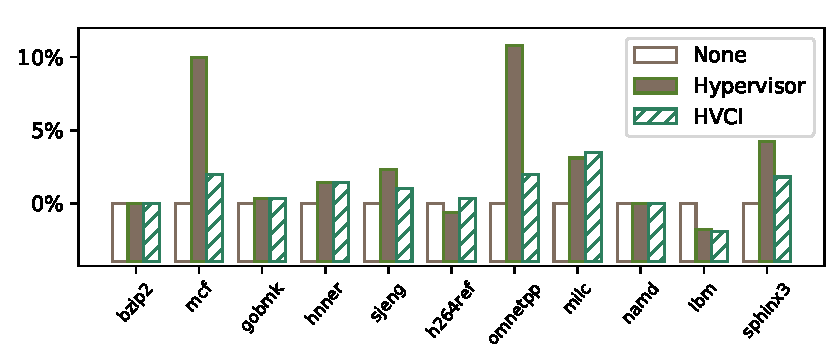
\includegraphics[width=0.47\textwidth]{figures/benchmark3}
  \centering
  \caption{Performance overhead on the SPEC benchmarks incurred by the run-time load hypervisor. HVCI represent the Windows 10 native hypervisor for Hypervisor-Protected Code Integrity. All overheads are normalized to the unprotected system running benchmark.}
  \label{fig:benchmark}
\end{figure}

We chose several non-trivial applications to demonstrate the performance overhead that introduced by our mitigation. 

\begin{figure}[th]
  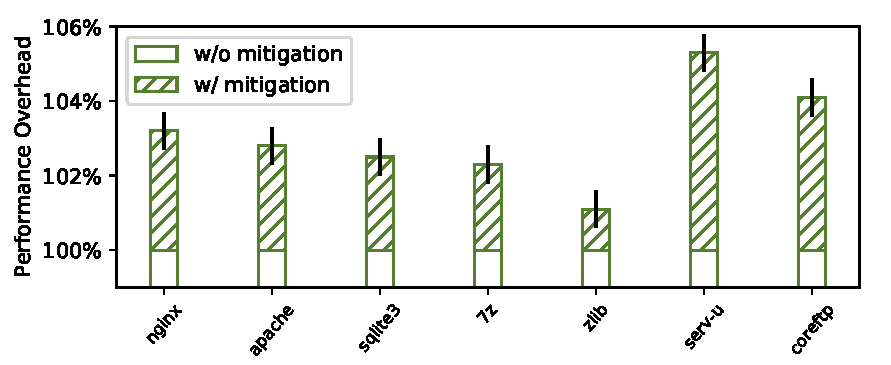
\includegraphics[width=0.47\textwidth]{figures/performance3}
  \centering
  \caption{Performance overhead in non-trivial applications. Overhead mostly being introduced on system calls that need to fetch user-mode parameters}
  \label{fig:performance}
\end{figure}

~\autoref{fig:performance} shows the performance overhead of our mitigation in several non-trivial application. Some of those applications potentially could be the trampoline service of kernel TOCTOU attacks.
For web server software such as Nginx. We test its performance by counting the accumulated response time for 10000 web requests. For compression software such as zlib, we test it with compressing large files. For sqlite3, we use speedtest1.c which is a common performance testing program.

The result shows that the performance overhead is modest. Because only the system calls that have user-mode buffer as their parameters will trigger SMAP exceptions. 

%Therefore the programs that have more system calls tends to have a higher performance overhead. We also count the ratio of SMAP exceptions to total page fault exceptions of one process.

% This is not correct, most page fault are caused by SMAP, following is the test results for nginx
%g_PagefaultCount 1000, g_PagefaultSMAPCount 992
%g_PagefaultCount 2000, g_PagefaultSMAPCount 1986
%g_PagefaultCount 3000, g_PagefaultSMAPCount 2982
%g_PagefaultCount 4000, g_PagefaultSMAPCount 3981
%g_PagefaultCount 5000, g_PagefaultSMAPCount 4980
%g_PagefaultCount 6000, g_PagefaultSMAPCount 5979
%g_PagefaultCount 7000, g_PagefaultSMAPCount 6978
%g_PagefaultCount 8000, g_PagefaultSMAPCount 7974
%g_PagefaultCount 9000, g_PagefaultSMAPCount 8968


Part of the overhead is introduced due to the overall intercepting of page fault exceptions of the system. The page fault handler is called in high frequency. Our page fault hook currently is installed directly in the IDT table of each processor. Hence every page fault exception goes through our handler. Even though, in the very begining, we pass through exceptions that doesn't belong to the target process, still extra instructions are executed for each exception.

%Although we use virtualization techniques, but the hypervisor we use is a very simple one. Unlike commercial virtualization solutions such as VMWare, Xen and Qemu+Kvm, ours doesn't emulate any hardware devices nor intercept further page mapping translate that between host and guest. Only several types of VM-Exit is inevitable such as control register accessing which we do need to handle it too.

\subsection{Case Study}

We write a proof-of-concept(POC) program to test our mitigation against CVE-2008-2252. It triggers the TOCTOU vulnerability to introduce a memory buffer overflow. 

%We test it on the Windows XP sp3 system with the vulnerable win32k.sys file whose version is 5.1.2600.5512. Because SMAP only available at Intel 5th generation CPU (architecture code name Broadwell). Hard-disk controller which integrated in the CPU corresponded chipset doesn't support ATA mode anymore, and Windows XP system doesn't support AHCI mode, so it's difficult to install it on a modern PC. Our testing environment is established using a virtual machine. Particularly, VMWare Workstation 14 Player, emulated "Intel Core i5-6200U CPU (2 cores) with 1GB of RAM", option "Virtualize Intel VT-x/EPT or AMD-v/RVI" also enabled.

The attacking program has two threads. The main thread first allocate a page at virtual address 0, which later used as the parameter to be sent into the vulnerable syscall. The reason to choose page zero is to bypass the parameter check in syscall NtUserMessageCall. Next, right after creating another thread, it keeps calling the vulnerable function SendMessage (WM\_COPYDATA) with the malicious parameters in a loop, which eventually calls the vulnerable win32k function xxxInterSendMsgEx. The created thread then keep modifying the parameter at page zero, also in a loop, simultaneously.

\begin{figure}[th]
  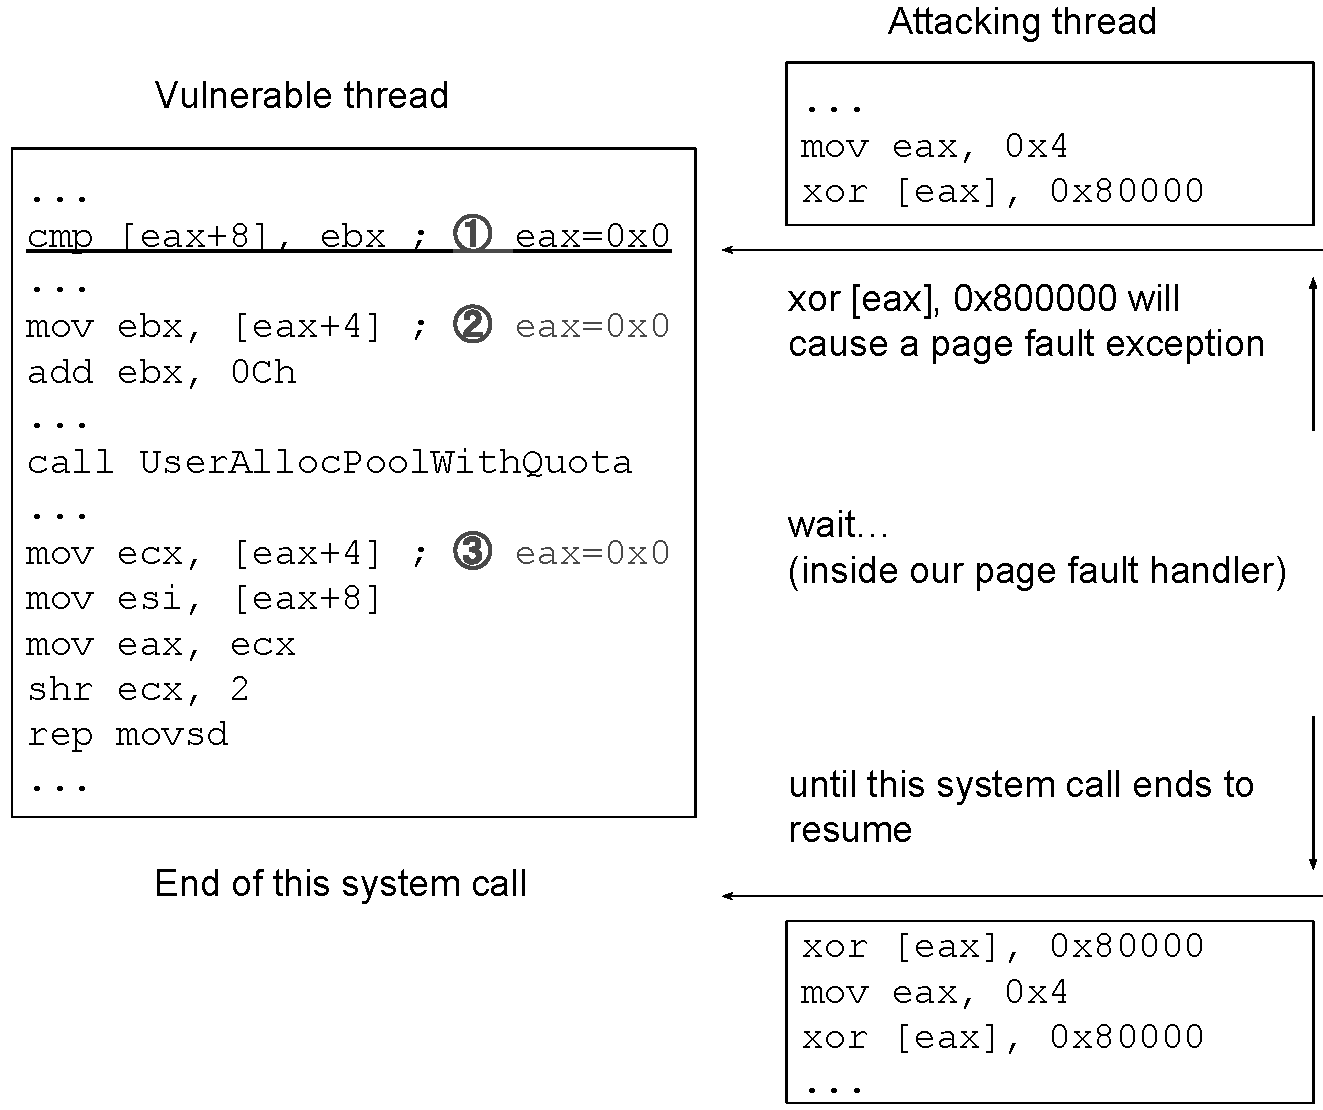
\includegraphics[width=0.47\textwidth]{figures/ms08061case}
  \centering
  \caption{The user page will be protected right at the moment it's been referenced.}
  \label{fig:ms08061case}
\end{figure}

In the attack, as shown in ~\autoref{fig:ms08061case}, the \textcircled{2} and \textcircled{3} are the places where vulnerable user-mode variable pcbData are referenced, it's address is 0x4. But the first time the zero page get accessed is \textcircled{1} where several instruction ahead of \textcircled{2}, it triggers an page fault exception (cased by SMAP). Therefore this page will be marked as a kernel page by our page fault handler. From this moment until the end of the current system call, this page will be protected from modifying by either as a kernel page or a user page with read-only permit. If the attacking thread try to modified it, another page fault exception  will be raised because of access violation. Then the attacking thread will be held for 30 milliseconds before it try to re-execute the faulting instruction again, for as many as 10 times. If not possible, the attacking thread will be terminated. We can see that during the protection, memory reads at \textcircled{2} and \textcircled{3} are kept consistent.


CVE-2013-1254 is another typical TOCTOU vulnerability that found in Windows win32k module~\cite{jurczyk2013identifying}. It effects both Windows XP and Windows 7. 

%A series of same kind of vulnerability found in 26 functions of module win32k.

\begin{lstlisting}[style=code] 
.text:BF8A993F   mov   eax, _W32UserProbeAddr
                       .
                       .
.text:BF8A9973   @cmp   [ecx+8], eax@    
.text:BF8A9976   jnb   short loc_BF8A997B
.text:BF8A9978   @mov   eax, [ecx+8]@    
.text:BF8A997B
.text:BF8A997B loc_BF8A997B:                           
.text:BF8A997B   mov   ecx, [eax]
.text:BF8A997D   mov   eax, [eax+4]
\end{lstlisting}
%\captionof{lstlisting}{Flawed code in win32k.sys function SfnINOUTSTYLECHANGE()}

The flawed function first fetch a value from "ecx+8" and compare it with \_W32UserProbeAddress which is a value that indicates the highest possible address for user-mode variables. It confirms that the variable is actually reside in user space. Next, it fetches the value again and assign it to eax. This is where the double fetch happens. The attacker can change the value between those two fetches, letting it bypass the verification,  then assign it a kernel space address.

So when "ecx+8" is referenced the first time, the corresponding page will trigger a SMAP exception, then this page will be protected until the current system call ends. Other threads write to it will also trigger page fault exceptions, as explained in the previous case, out page fault handler will handle those to keep the data consistent. 


